By applying computing to all kinds of areas, information technology (IT) has been transforming the way we 
understand and change the world. Over the past few decades, IT has realized the fast analysis of massive 
quantities of data and the rapid transmission of tremendous amount of information, facilitating 
countless advances in areas of science and technology. 
%enable the solution of vastly more accurate predictive models and the analysis of massive quantities of data, 
%producing quantum advances in areas of science and technology.
As our reliance on IT continues to increase, the complexity and urgency of the problems our society will face 
in the future necessitate the building of more powerful and ubiquitous computing systems. 

Since CPU frequency flattened out in early 2000s, parallelism from all levels has become the ``golden rule" to boost performance 
in the computer industry. Among the different types of modern computing systems, large-scale High Performance 
Computing (HPC) and Cloud Computing systems are the two most powerful ones. 
For both of them, the extraordinary computing capacity attributes to a massive amount of parallelism, which is achieved by 
equipping the system with hundreds or thousands of CPUs, accelerators, communication devices, storage components, etc. 


With the increase in the number of components, it become more and more challenging for 
researchers to continually offer more computing capacity with sustainable performance and reliability. 
As today's HPC and Cloud systems grow to 
meet tomorrow's demands, the behavior of the systems will be increasingly difficult to specify, predict and manage. 
This upward trend, in terms of scale and complexity, has a direct negative effect on the overall system reliability. 
%Even with the expected improvement in the reliability of future computing technology, the rate of system level failures will 
%dramatically increase with the number of components, possibly by several orders of magnitude. 
At the same time, the rapid growing power consumption is another major concern. 
It is reported that 
the power required to run the machines as well as cool them has become the largest cost factor in a large-scale system's operating 
expenses~\cite{scaramella2014worldwide}.  
In future-generation large-scale computing systems, failure would become a norm rather than an exception, 
driving the system to significantly lower efficiency with unprecedented amount of power consumption. 

%Since CPU frequency flattened out in early 2000s, parallelism has become the ``golden rule" to boost performance. 
%In HPC, Terascale performance was achieved in the late 90’s with fewer than 10,000 heavyweight single-core processors. 
%A decade later, petascale performance required about ten times more processors with multiple cores on each processor. Nowadays, a race
%is underway to build the world's first exascale machine to accelerate scientific discoveries and breakthroughs. It is 
%projected that an exascale machine will achieve billion-way parallelism by using one million sockets each supporting 
%1,000 cores~\cite{doe_ascr_exascale_2011,top_ten_2014}. 
%
%Similar trend is happening in Cloud Computing. 
%As the demand for Cloud Computing accelerates, cloud service providers  
%will be faced with the need to expand their underlying infrastructure to ensure the expected levels of performance, reliability and cost-effectiveness. 
%As a result, lots of large-scale data centers have been and are being built by IT companies
%to exploit the power and economies of scale. 
%For example, Google, Facebook, and Rackspace have hundreds of thousands 
%of web servers in dedicated data centers to support their business. 
%
%Unfortunately, several challenging issues come with the increase in system scale. As today's HPC and Cloud Computing systems grow to 
%meet tomorrow's compute power demand, the behavior of the systems will be increasingly difficult to specify, predict and manage. 
%This upward trend, in terms of scale and complexity, has a direct negative effect on the overall system reliability. 
%%Even with the expected improvement in the reliability of future computing technology, the rate of system level failures will 
%%dramatically increase with the number of components, possibly by several orders of magnitude. 
%At the same time, the rapid 
%growing power consumption, as a result of the increase in system components, is another major concern. 
%%It is reported that 
%%the power required to run the machines as well as cool them has become the largest cost factor in a large-scale system's operating 
%%expenses.  
%At future extreme-scale, failure would become a norm rather than an exception, 
%driving the system to significantly lower efficiency with unprecedented amount of power consumption. 

\section{Extreme-scale Computing}

Nowadays, large-scale computing systems are embracing two transformative trends, i.e., the rapid growth
in HPC with in particular an international
exascale initiative, and the dramatic expansion of Cloud infrastructures accompanied by the Big Data explosion. 
With concerted efforts from researchers in various disciplines, a race
is underway in the HPC community to build the world's first exascale machine, featuring a computing capability of exaFLOPS, 
to accelerate scientific discoveries and breakthroughs. It is 
projected that within the next decade an exascale machine will achieve billion-way parallelism by using one million sockets each supporting 
1,000 cores~\cite{doe_ascr_exascale_2011,top_ten_2014}. 

Similarly, remarkable expansion is happening in Cloud Computing.  
Due to its incomparable advantages, such as low entry cost and on demand resource provisioning, 
Cloud Computing has become the fastest growing segment in the software industry~\cite{anderson2013forecast}.
As the demand for Cloud Computing accelerates, cloud service providers  
will be faced with the need to expand their underlying infrastructure to ensure the expected levels of performance, reliability and cost-effectiveness. 
As a result, numerous large-scale data centers have been and are being built by IT companies
to exploit the power and economies of scale. 
For example, Google and Rackspace have hundreds of thousands 
of web servers in dedicated geo-distributed data centers to support their business. 

The path to future extreme-scale computing involves several major roadblocks and numerous challenges inherent 
to the complexity and scale of these systems. 
The system scale needed to address our future computing needs will come at the cost of increasing unpredictability  
and operating expenses. As we approach extreme-scale, two of the biggest challenges will be power 
consumption and system resilience, both being direct consequences of the dramatic increase in the 
number of system components~\cite{exa_challenge_2010,snir2014addressing}. 

As a result of the continuous growth in system scale, there has been a steady rise in power consumption in large-scale systems. 
Google engineers, operating thousands of servers, warned that if power consumption continues to grow, power costs can easily overtake hardware costs by a large margin~\cite{barroso2005price}. Figure~\ref{fig:top_500_power} reveals the same concern in supercomputers. 
In 2005, the peak power consumption of a single supercomputer reached 3.2 Megawatts (MW). This number was doubled only after 5 years, and 
further climbed to 17.8 
MW in 2013 with a machine of 3,120,000 cores~\cite{top500}. Recognizing this upward trend, the U.S. Department of Energy has set 20 
MW as the power limit for future exascale systems, so that a power budget of \$20 million per year is preserved for any supercomputer~\cite{doe_ascr_exascale_2011}. 
%challenging the research community to provide a 1000x improvement in performance with only a 10x increase in power~\cite{exa_challenge_2010}. 
%This huge imbalance makes system power a leading design constraint on the path to exascale. 
Although largely pragmatic, this constraint challenges the HPC community to design future systems capable of sustaining 50 GFlops
per Watt (GF/W). According to the Green500 list released in June 2017, the most energy-efficient supercomputer is the new TSUBAME 3.0 at the Tokyo Institute 
of Technology~\cite{top500}. It achieved 14.110 GF/W during its 1.998-petaflop Linpack performance run. To enable future exascale system, 
combined efforts from hardware, OS, and software must improve energy efficiency by a factor of over 3.5X, making system power a leading design constraint on the path to exascale. 

\begin{figure}[t]
	\begin{center}
		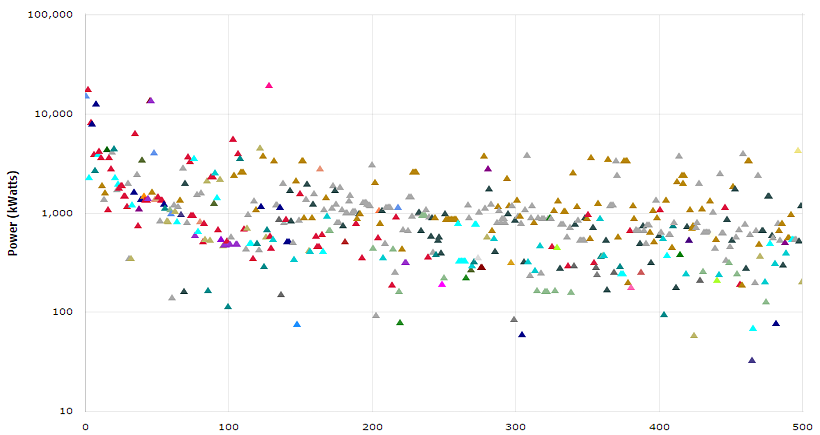
\includegraphics[width=0.9\textwidth]{Figures/top_power}
	\end{center}
	\caption{System power consumption of the top 500 supercomputers as of June 2017~\cite{top500}.}
	\label{fig:top_500_power}
\end{figure}

%\begin{figure}[t]
%	\begin{center}
%		\subfigure[System power consumption]
%		{
%			\label{fig:top_power}
%			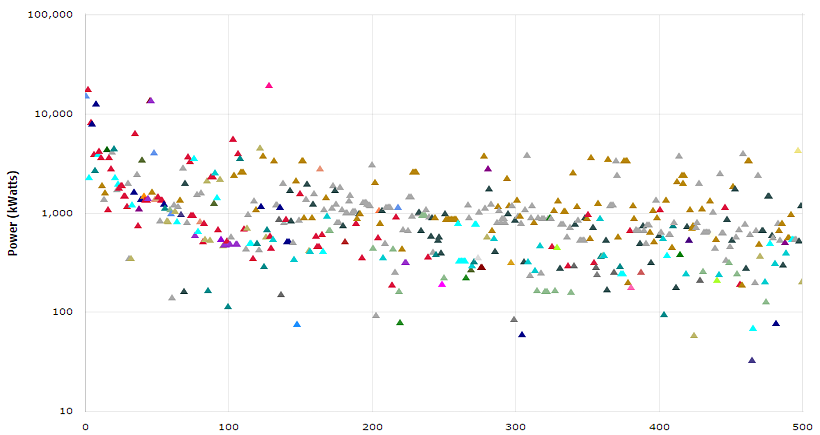
\includegraphics[width=0.8\textwidth]{Figures/top_power}
%		}
%		\subfigure[System power efficiency]
%		{
%			\label{fig:top_power_effi}
%			\includegraphics[width=0.8\textwidth]{Figures/top_power_effi}
%		}
%	\end{center}
%	\caption{Distribution of the system power consumption and power efficiency of the top 500 supercomputers as of June 2017. The highest power record is achieved by QUARTETTO at 19,431 kW. The highest power efficiency is achieved by TSUBAME 3.0 at 14.110 GF/W~\cite{top500}.}
%	\label{fig:top_500_power}
%\end{figure}

Due to the expected complexity and scale of future extreme-scale systems, another major roadblock is the increasing propensity of the system to diverse types of failures. 
Regardless of the reliability of individual component, the system level failure rate will continue to increase as the number of 
components increases, possibly by several orders of magnitude. It is projected that the Mean Time Between Failures (MTBF) of future extreme-scale systems will be at the order of hours or even minutes, implying 
that many failures will occur every day~\cite{Bergman08exascalecomputing}. Without an efficient fault tolerance mechanism, faults will be so frequent that the applications running on the 
systems will be continuously interrupted and restarted.%, greatly slowing down the application progress. 

Today, fault tolerance in computing systems mainly relies on rollback recovery, which rolls back and restarts the execution 
every time there is a failure. This approach is often equipped with checkpointing to periodically save the execution state to a 
stable storage, so that execution can be restarted from a recent checkpoint in the case of a failure~\cite{Elnozahy:02:Survey,kalaiselvi_sadhana_2000,chandy_trans_1985}. 
Although checkpoint/restart is the most widely used technique in today's HPC systems, several studies predict that it is not likely to scale to future extreme-scale systems~\cite{ferreira_sc_2011,elnozahy_dsc_2004,4367962}. 
Table~\ref{tbl:cp_effi} shows that at 100k nodes, only 35\% of the time will be spent on useful work, while 55\% of the time will be wasted on checkpointing and restarting. 
Given the anticipated increase in system level failure rates and the time to checkpoint large-scale 
compute-intensive and data-intensive applications, the time required to periodically checkpoint an application 
and restart its execution will approach the system's MTBF~\cite{Cappello:2009:TER:1640402.1640428}. Consequently, applications will make little forward progress, thereby 
reducing considerably the overall system efficiency and wasting a lot of energy. Furthermore, the nature and diversity of failures in extreme-scale systems are such that checkpoint/restart alone may not be an adequate approach. Based on this observation, recent work has proposed state machine replication as a scalable solution to handling diverse types of faults~\cite{fiala_2012_sdc,ferreira_sc_2011}. 

\begin{table}
\centering
\caption{Projection of time spent on each part when using checkpoint/restart to guard a 168-hour job at different system scales~\cite{fiala_2012_sdc}. 5 years MTBF per node, 15 minutes checkpoint time. Optimal checkpoint interval is derived using Daly's model~\cite{daly_fgcs_2006}. }
\label{tbl:cp_effi}
\begin{tabular}{r c c c c} 
 \hline
 \# Nodes  & work & checkpoint & recompute & restart \\
 \hline\hline
 100 & 96\% & 1\% & 3\% & 0\% \\
1,000 & 92\% & 7\% & 1\% & 0\% \\
10,000 & 75\% & 15\% & 6\% & 4\% \\
100,000 & 35\% & 20\% & 10\% & 35\% \\  
 \hline
\end{tabular}
\end{table}
State machine replication exploits hardware redundancy and executes multiple instances of a task across compute nodes 
in parallel to overcome failure~\cite{bartlett_1981_nonstop,tsai_isads_2011,ferreira_sc_2011}. Although this approach is extensively used 
to deal with failures in 
Cloud Computing and mission critical systems, it has 
never been used in any production HPC system due to its waste of resources. To replicate each process, state machine replication not only requires 
twice the amount of compute nodes at least, but also increases the power consumption proportionally, which might exceed any imposed power budget. 

Based on above analysis, neither of the two existing approaches would efficiently tolerate failure for future extreme-scale systems. And unfortunately, neither 
of them addresses the power cap issue. 
Therefore, achieving high resilience to failures under strict power constraints is a daunting and critical challenge that requires new 
fault tolerance models with scalability and power-awareness in mind. 
 
\section{Research Overview}

There is a delicate interplay between fault tolerance and power consumption. Process replication and checkpoint/restart require 
additional power to achieve fault tolerance. Conversely, it has been shown that lowering supply voltages, a commonly used 
technique to conserve power, increases the probability of transient faults~\cite{chandra2008defect,zhao2008reliability}. The trade-off between fault free operation and 
optimal power consumption has been explored in the literature~\cite{meneses2014energy,mills2014energy}. Limited insights have emerged, however, with respect to how 
adherence to application's desired QoS requirements affects and is affected by the fault tolerance and power consumption 
dichotomy. In addition, abrupt and unpredictable changes in system behavior may lead to unexpected fluctuations in performance, 
which can be detrimental to applications’ QoS requirements. The inherent instability of extreme-scale computing systems, 
in terms of the envisioned high-rate and diversity of faults, together with the demanding power constraints under which 
these systems will be designed to operate, calls for a 
reconsideration of the fault tolerance problem.

To this end, this thesis aims at developing a novel fault-tolerant computational model that simultaneously addresses the power and resilience challenges for emerging extreme-scale computing systems. Our goal is to study the viability of and provide the justification for the following \textbf{thesis statement}: 

\vskip 10pt
\textit{``It is possible to persistently achieve Quality of Service  with sustainable system efficiency, while operating under diverse types of failures and stringent power constraints, in future extreme-scale computing systems."}
\vskip 10pt

We seek to achieve this objective by developing an adaptive and power-aware fault tolerance model, referred to as \textit{Leaping Shadows}. It builds on top of the recently proposed Shadow Replication model, and exploits novel techniques to address the limitations of Shadow Replication to meet the performance and resilience requirements of extreme-scale computing. With an extensive evaluation through the combination of analytical models and empirical experiments, this thesis demonstrates the viability of Leaping Shadows to achieve high tolerance to failure that is more time and energy efficient that state-of-the-art approaches.

The basic tenet of Shadow Replication is to associate with each original process a suite of coordinated ``shadow processes", whose size depends on the criticality of the application and its QoS requirements. To tolerate failure while minimizing energy, the shadows are scheduled to execute in parallel with the original process, but on different nodes and at reduced rates. A shadow is an exact replica of its associated original process. If an original process fails, one of the associated shadows takes over and resumes the execution, with a potential increase in execution rate to mitigate delay. 


Relying on Dynamic Voltage and Frequency Scaling (DVFS) to control execution rates, 
Mills studied the execution dynamics of Shadow Replication and its performance in HPC systems~\cite{mills_2014_icnc,mills_2014_pdp,mills2014power}. Through the use of modeling, simulation, and experimentation, Mills demonstrated that Shadow Replication can achieve resilience more efficiently than both checkpoint/restart and traditional state machine replication when power is limited. %However, in Mills' work, execution rate control in Shadow Replication is limited to the use of DVFS, which has been shown to have various issues that question its viability~\cite{Eyerman:2011:FDU:1952998.1952999,Keller:EECS-2015-257,chandra2008defect,zhao2008reliability}. In addition, Mills' study is limited to HPC systems and focuses exclusively on minimizing energy consumption with constraints on time to completion. In contrast, QoS requirements can be expressed in multiple dimensions that go beyond time and energy. Last but not least, the Shadow Replication model has several drawbacks that impact performance, expose vulnerability, and limit fault tolerance capability in extreme-scale, failure-prone computing environments.
However, Mills' study is limited to HPC systems and focuses exclusively on minimizing energy consumption with constraints on time to completion. In contrast, QoS requirements can be expressed in multiple dimensions that go beyond time and energy. Furthermore, the Shadow Replication model has several drawbacks that impact performance, expose vulnerability, and limit fault tolerance capability in extreme-scale, failure-prone computing environments.

To address the above limitations, this thesis builds on the computational model of Shadow Replication, and seeks to tolerate high rate of diverse types of failures in emerging power-constrained HPC and Cloud systems, while guaranteeing system efficiency and application QoS.
Specifically, we have complemented Mills' work by developing analytical models and optimization frameworks for different objectives in the Cloud environments~\cite{cui_2014_closer}. This work demonstrates Shadow Replication's adaptivity in balancing the trade-offs among performance, power, and resilience, and highlights its flexibility in achieving multi-dimensional QoS requirements. Additionally, we have proposed and studied the Leaping Shadows model which is depicted in Figure~\ref{fig:block_diagram}. Leaping Shadows  exploits novel techniques of shadow collocation, leaping, and rejuvenation to address the \textit{divergence} and \textit{vulnerability} issues with Shadow Replication. Furthermore, we have applied Leaping Shadows to tolerate Silent Data Corruption (SDC), which is another class of failure that has become prevalent in current large-scale systems~\cite{fiala_2012_sdc}. Last but not least, a prototype of Leaping Shadows in Message Passing Interface (MPI) has been implemented, to validate the computational model as well as measure its performance in real environments. 

\afterpage{
\begin{figure}[t]
	\begin{center}
		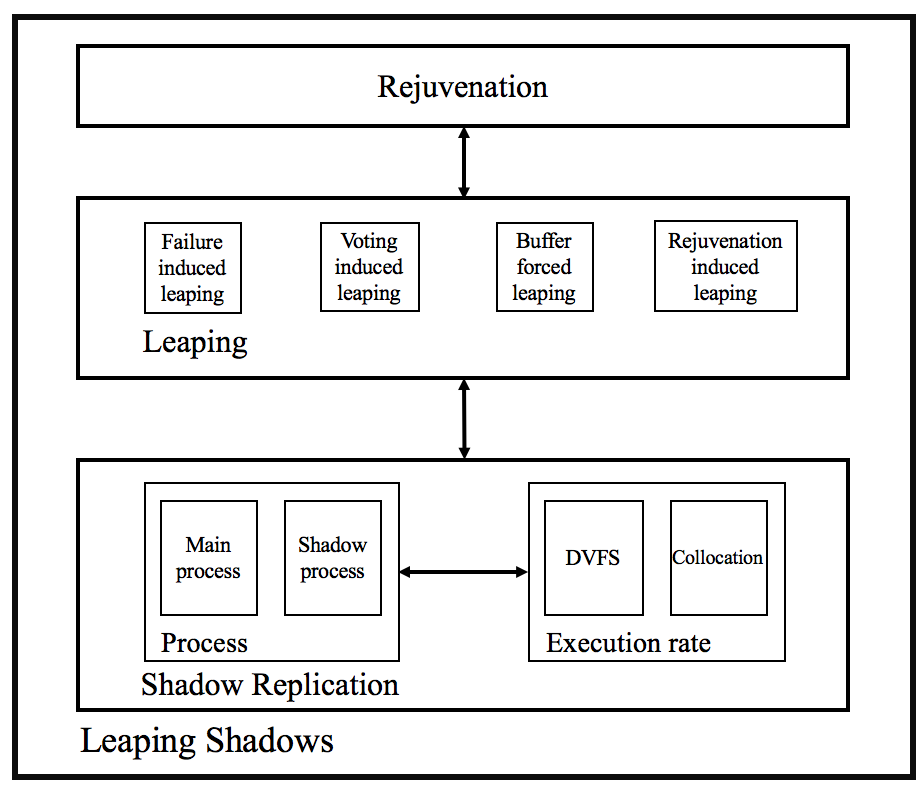
\includegraphics[width=\textwidth]{Figures/block_diagram}
	\end{center}
	\caption{Overview of the Leaping Shadows computational model.}
	\label{fig:block_diagram}
\end{figure}
\clearpage
}
\subsection{Contributions}
This thesis consists of the following main contributions.

\textbf{Reward-based optimal Shadow Replication}.
Shadow Replication is an adaptive and flexible computational model that can achieve multi-dimensional QoS requirements. 
The major challenge resides in determining jointly the execution rates of all task instances, 
both before and after a failure occurs, with the objective to optimize performance, resilience, power consumption, or their combinations.
In this work we focus on the Service Level Agreement (SLA) requirements in the Cloud and develop a reward-based analytical framework, in order to derive the optimal execution rates for maximizing reward and minimizing energy 
costs under strict completion time constraints~\cite{cui_2014_closer,cui_en7085151}. 


\textbf{The Leaping Shadows model}.
Enabling Shadow Replication for resiliency in extreme-scale computing brings about a number of challenges and design decisions, including the applicability of this concept to a large number of tasks executing in parallel, 
the effective way to control shadows’ execution rates, and maintenance of consistent resilience through a large number of failures. Taking into consideration the main characteristics of compute-intensive and 
highly-scalable applications, 
we devise novel ideas of shadow collocation, leaping, and rejuvenation, and integrate them with Shadow Replication to establish a more efficient and scalable model of Leaping Shadows~\cite{cui_2016_scalcom}.

\textbf{Tolerance of Silent Data Corruption (SDC) with extended Leaping Shadows}.
Different from crash failures, which terminate the execution on a faulty processor, SDC allows a faulty processor to continue to completion but may silently generate incorrect results. In order to detect and correct a single SDC, Leaping Shadows associates 2 shadows with each main process. The primary shadow is scheduled to run at the same rate as its associated main, so that voting can be used to detect SDC in a timely manner, and correct results can be confirmed if no SDC. In order to minimize energy, the secondary shadow initially executes at a reduced rate. As a result, it can also benefit from leaping to achieve forward progress with minimal overhead. Based on this idea, we have established precise analytical models and optimization frameworks to
quantify and optimize the performance. 

\textbf{A proof-of-concept implementation of Leaping Shadows in MPI}.
Though Leaping Shadows has been evaluated analytically, a real implementation 
is needed for validation and performance measurement in real systems. We have developed \textit{lsMPI} as a prototype of Leaping Shadows in Message Passing Interface (MPI), which is the de facto programming paradigm for HPC. 
Instead of a full implementation of MPI, the library is designed to be a separate layer between MPI runtime and user application, in order to take advantage of existing MPI performance optimizations that numerous researches have spent years on. 
This implementation transparently spawns 
a shadow for each main process during the initialization phase, manages the coordination between mains and shadows, 
and guarantees order and consistency for messages and non-deterministic events. 
In addition, we have implemented leaping and rejuvenation to efficiently tolerate a large number of crash failures. 


\textbf{Performance evaluation of Leaping Shadows}.
With the lsMPI implementation, extensive experiments have been conducted to measure its real system performance, using benchmark applications that represent a wide range of HPC workloads. As a first step, we measured the failure-free runtime overheads resulted from the enforced consistency protocol. This experiment reveals that the overheads depend on application, and vary from 0.64\% to 2.47\%. Then we measured the scalability in order to predict the performance at extreme-scale, which suggested that the overheads would remain under 8\% at $2^{20}$ processes. Lastly, we also implemented in-memory checkpoint/restart to compare with lsMPI in the presence of failures. The results demonstrate Leaping Shadows'
ability to tolerate high failure rates, and to outperform in-memory checkpoint/restart in both execution time and
resource utilization.

\section{Thesis Outline}
\label{outline}
The rest of this thesis is organized as follow:  
Chapter \ref{chapter:background} reviews literature. It provides a background study of existing fault tolerance and power management techniques in large-scale computing systems. 
Chapter \ref{chapter:shadowing} introduces the Shadow Replication computational model, which forms the foundation of this work. In Chapter \ref{chapter:reward}, we build a reward-based optimization framework for Shadow Replication in the Cloud environment.
In Chapter \ref{chapter:scale}, we introduce the Leaping Shadows model, which addresses the shortcomings of Shadow Replication in failure-prone, extreme-scale systems. 
Tolerance of silent data corruption is discussed in Chapter \ref{chapter:sdc}.
Chapter \ref{chapter:implementation} presents the details of a Leaping Shadows implementation as well as its performance evaluation. 
Finally, Chapter~\ref{chapter:summary}  concludes the thesis.








